Мирко и Славко играют с игрушечными зверюшками. Сначала они выбирают одну из трех возможных
досок для игры, показанных на рисунке ниже. Каждая доска состоит из ячеек (показанных ниже
кружками), организованных в одно-, двух- или трехмерную решетку. 

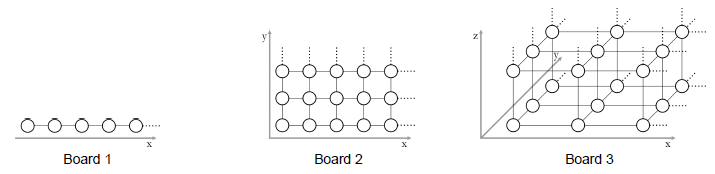
\includegraphics[scale=0.9]{pairs.png}

Затем Мирко размещает $N$ зверюшек по ячейкам. 

Расстояние между двумя ячейками~--- это минимальное количество ходов, которое потребовалось бы
зверюшке, чтобы переместиться из одной из этих ячеек в другую. За один ход зверюшка может
переместиться в любую из соседних ячеек (на рисунке соседние ячейки соединены отрезками).

Две зверюшки могут слышать друг друга, если расстояние между их ячейками не превосходит числа $D$.
Задача Славко~--- подсчитать количество пар зверюшек, которые могут слышать друг друга. 

Напишите программу, которая по заданному типу доски, положению всех зверюшек на ней и числу $D$ находит требуемое количество пар зверюшек. 